\documentclass[a4paper,11pt]{article}
\usepackage[utf8]{inputenc}
\usepackage[italian]{babel}
%\usepackage[top=3 cm, bottom=3.5 cm, left=2.5 cm, right=2.5 cm]{geometry}
\usepackage{siunitx}
\usepackage{fancyhdr}
\usepackage{amsthm}
\usepackage{amsmath}
\usepackage{amssymb}
\usepackage{graphicx}
\usepackage{float}
\usepackage{braket}
%\usepackage{tikz}
\usepackage{rotating}
\usepackage{subfigure}
%\usetikzlibrary{decorations}
%\usetikzlibrary{er}
\graphicspath{{./img/}}

\author{Ruggero Lot \\ ruggero90@gmail.com \\ fisica della materia \\}
\title{Esame di MBS}
\begin{document}
	\maketitle
	\paragraph{Problema:} % (fold)
	\label{par:problema}
		Si consideri un cristallo LJ con un interstiziale: ovvero una struttura
		FCC di N siti cristallini occupati da N+1 atomi, l' N+1-mo trovandosi in
		un sito non FCC. Si ponga l'atomo addizionale in modo da massimizzare la
		distanza dai primi vicini (il cristallo sarà sotto stress, si calcoli la
		struttura di equilibrio usando uno Steepest Descent).\\
		L'obiettivo è di calcolare il coefficiente di autodiffusione D, il quale,
		visto che il cristallo perfetto praticamente non diffonde, sarà dovuto 
		interamente all'atomo addizionale. Può essere che per vedere una diffusione
		apprezzabile sia necessario avvicinarsi alla T di fusione, facendo
		attenzione a verificare che il sistema rimanga solido (calcoli affini
		nello stato liquido possono essere d'aiuto). A questo fine può essere
		utile partire da T relativamente basse per poi eseguire simulazioni a T
		via via più alte, ogni volta partendo dallo stato finale della simulazione
		precedente.\\
		Eseguire un fit di $D(T)$ seguendo la relazione di Arrhenius
		\begin{equation*}
			D = D_0 e^{\frac{Q}{kT}}. 
		\end{equation*}
		Stimare la dipendenza di D da N per almeno una T.
	% paragraph problema (end)
	\newpage
	\tableofcontents
	\newpage
	\section{Software per la creazione del Sample} % (fold)
	\label{sec:software_per_la_creazione_del_sample}
		Il software ``starting\_positions'' è stato scritto allo scopo di poter 
		generare un campione sul quale andare poi ad eseguire simulazioni per
		raccogliere dati sul comportamento delle particelle.\\
		Il campione generato attraverso questo strumento consiste in un reticolo
		FCC (di passo reticolare a piacere) con un atomo interstiziale(se 
		richiesto) contenuto in una scatola cubica (di lato l) e pronto per
		essere utilizzato in algoritmi capaci di implementare le condizioni 
		periodiche al contorno.\\
		Il software consta di 2 algoritmi: il primo è quello di posizionamento 
		delle particelle all'interno della scatola, operazione che viene svolta
		in maniera sequenziale inserendo i 4 atomi per ogni cella unitaria nelle 
		posizioni FCC con la base:
		\begin{align}
			\mathbf a_1  &= a(0,0,0) & 
			\mathbf a_2  &= a(0,0.5,0.5) &
			\mathbf a_3  &= a(0.5,0,0.5) 
		\end{align}
		scartando eventuali atomi esterni alla scatola o doppi a causa delle pbc.\\
		Il secondo invece si occupa di portare il sistema, se sotto stress, ad uno 
		stato di equilibrio. Per risolvere questo problema è stato utilizzato uno 
		Steepest Descent che consiste in tre operazioni cicliche: 
		\begin{itemize}
			\item calcolare il gradiente della funzione da minimizzare
			\item scendere lungo il gradiente fino a quando non si incontra un inversione nella pendenza
			\item verificare che la variazione di energia sia più piccola di un $\epsilon$ desiderato se si uscire se no ricominciare da capo
		\end{itemize}
	    Questo metodo non è molto rapido ma ci permette di ottenere comunque
	    risultati ragionevoli in tempi contenuti.
	    Nota importante, è stata inserita una normalizzazione del vettore di discesa
	    per evitare, soprattutto nelle fasi iniziali dove il vettore gradiente ha 
	    modulo molto grande, salti spaziali delle particelle privi di significato fisico.
	\subsection{Dati ottenuti} % (fold)
	\label{sub:dati_ottenuti}
		questo primo programma è stato fatto eseguire con dei valori numerici 
		pensati in modo tale da garantire immediatamente una situazione di stabilità
		del sistema eccezion fatta per la particella interstiziale che viene posizionata in maniera del tutto casule all'interno della scatola.
		\paragraph{Cella unitaria e scatola di simulazione\\} % (fold)
		\label{par:cella_unitaria_e_scatola_di_simulazione}
			Per la cella unitaria è stata valutata la situazione di maggior 
			stabilità: il potenziale di LJ
			\begin{equation}
				U(\mathbf{r}_{ij})= 4 \epsilon \left(\left(\frac{\sigma}{\mathbf{r}_{ij}}\right)^{12}\
				-\left(\frac{\sigma}{\mathbf{r}_{ij}}\right)^6\right)
			\end{equation}
			ha un minimo in:
			\begin{equation}
				\left|\mathbf{r}_{ij}\right| = 2^{\frac{1}{6}} \sigma
				\approx 2.12 \sigma
			\end{equation}
			pertanto il lato della cella FCC risulta essere, ponendo $\sigma = 1$:
			\begin{equation}
				l = \frac{2^{\frac{1}{6}+1}}{\sqrt{2}} \approx 1.59
			\end{equation}
			per la nostra scatola cubica sono stati scelti valori di lato pari a 
			$2l$, $3l$, $4l$, $5l$ che sono capaci di contenere rispettivamente: 
			$32$, $108$, $256$, $512$ particelle
		% paragraph cella_unitaria_e_scatola_di_simulazione (end)
		\paragraph{Evoluzione dell'energia durante lo Steepest Descent\\} % (fold)
		\label{par:evoluzione_dell_energia_durante_lo_steepest_descent}
			\`E comune osservare in tutti i grafici come l'energia sia molto
			elevata all'inizio e tenda rapidamente ad un valore molto piccolo per
			poi mantenersi quasi stabile.\\
			Questo è dovuto al fatto che la particella aggiunta in maniera 
			completamente casuale si trova quasi sempre vicino ad un altra 
			particella e il potenziale di ordine 12 fa si che anche piccoli
			spostamenti (i primi steps) causino grandi variazioni di energia;
			raggiunta in seguito una configurazione stabile questo 
			fenomeno sparisce.\\
			\begin{figure}[H]
					\centering
					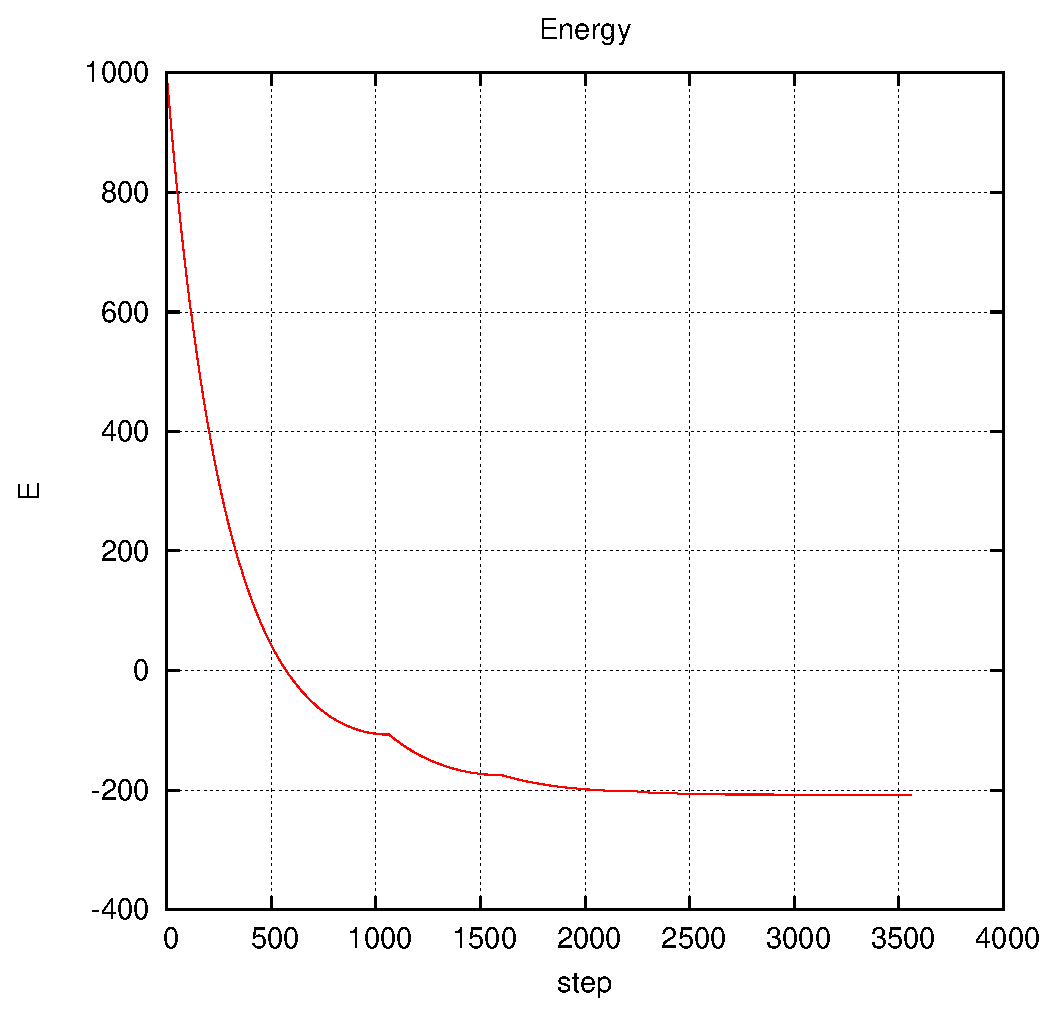
\includegraphics[scale = 0.7]{E_SD_32.eps}
					\caption{andameto dell'energia durante lo Steepest Descent per il campione composto da 32 particelle. Si notano chiaramente i cambi di direzione del gradiente e si osserva come la convergenza non impieghi molti step}
					\label{fig:SD_32}
			\end{figure}

			\begin{figure}[H]
				\centering
				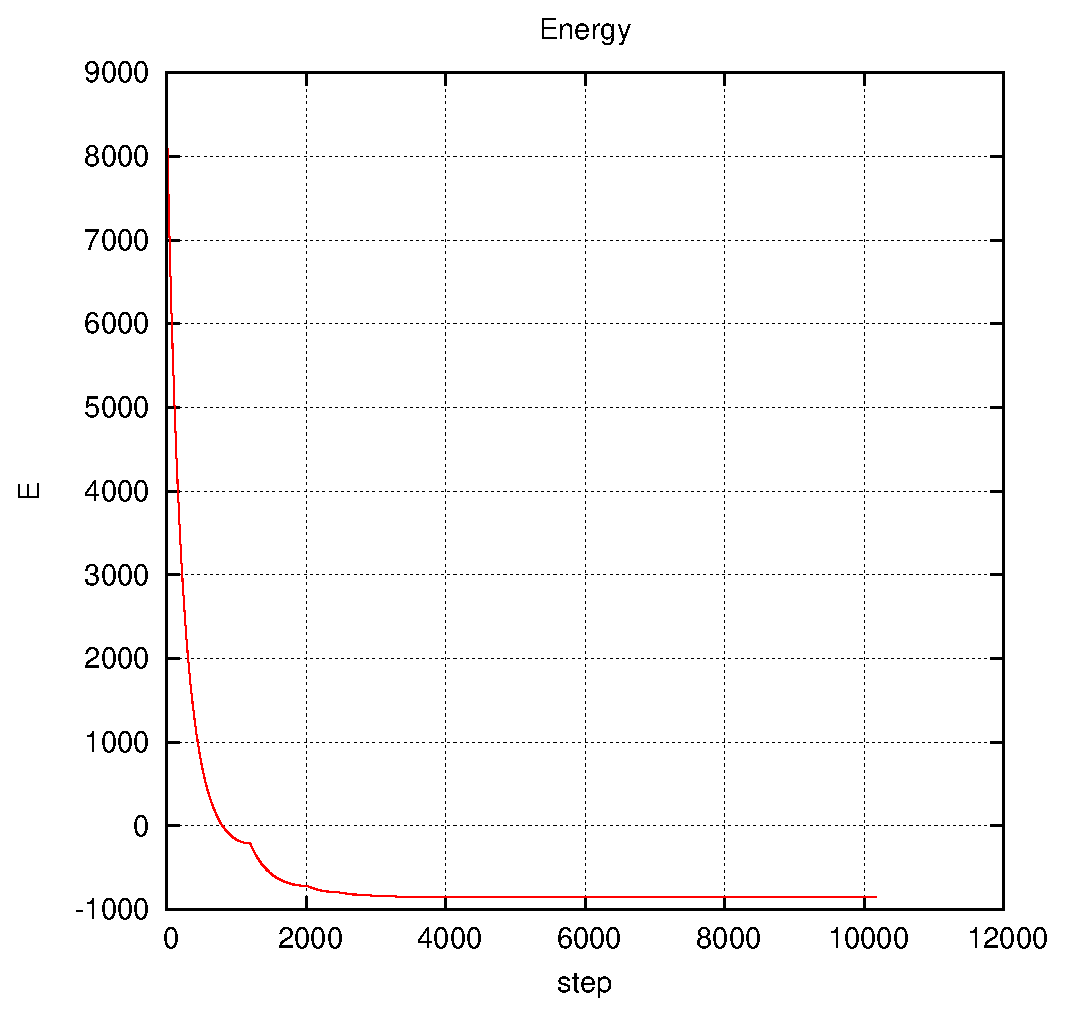
\includegraphics[scale=0.7]{E_SD_108.eps}
				\caption{andameto dell'energia durante lo Steepest Descent per il campione composto da 108 particelle. Si osserva comportamento simile alla figura \ref{fig:SD_32}}
				\label{fig:SD_108}
			\end{figure}
			\begin{figure}[H]
				\centering
				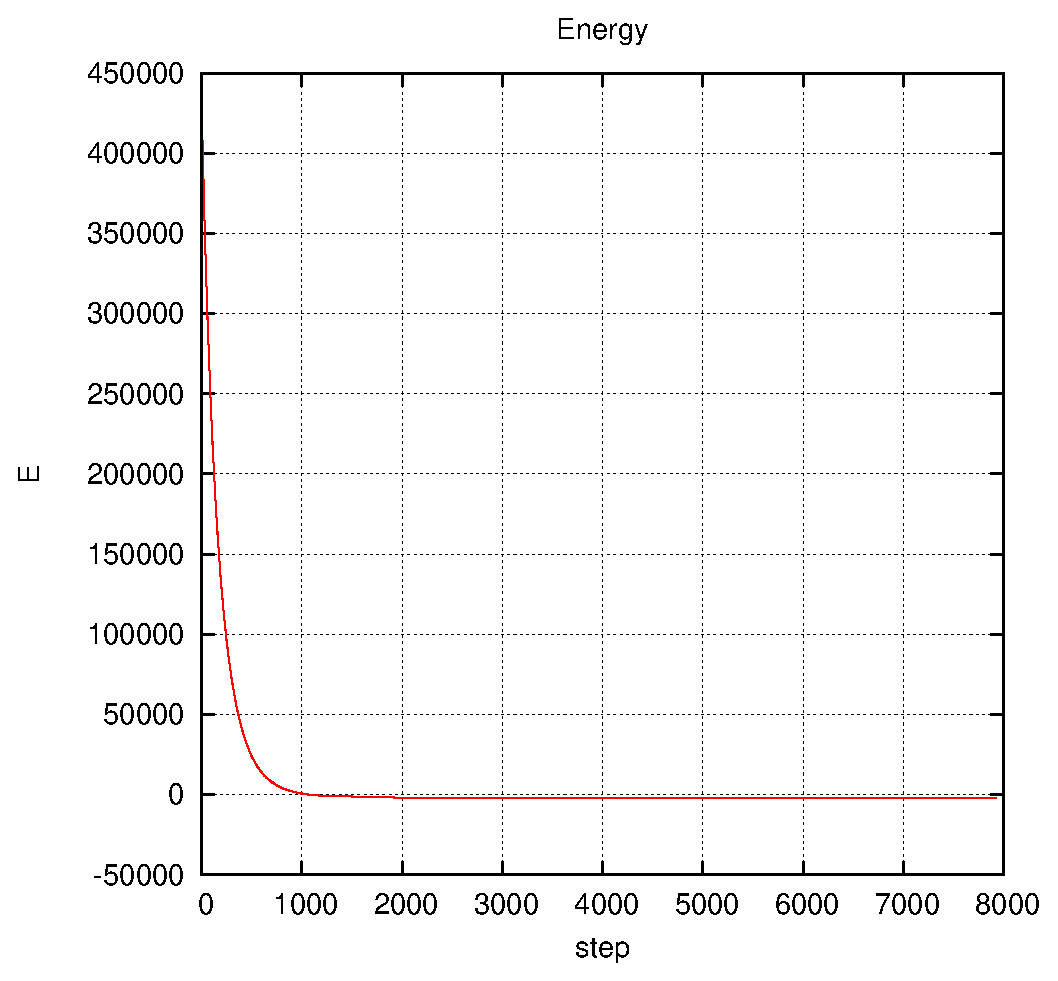
\includegraphics[scale=0.7]{E_SD_256.eps}
				\caption{andameto dell'energia durante lo Steepest Descent per il campione composto da 256 particelle. Qua si perde la concezione di cambio del gradiente in quanto i punti sono troppo fitti.}
				\label{fig:SD_256}
			\end{figure}
			\begin{figure}[H]
				\centering
				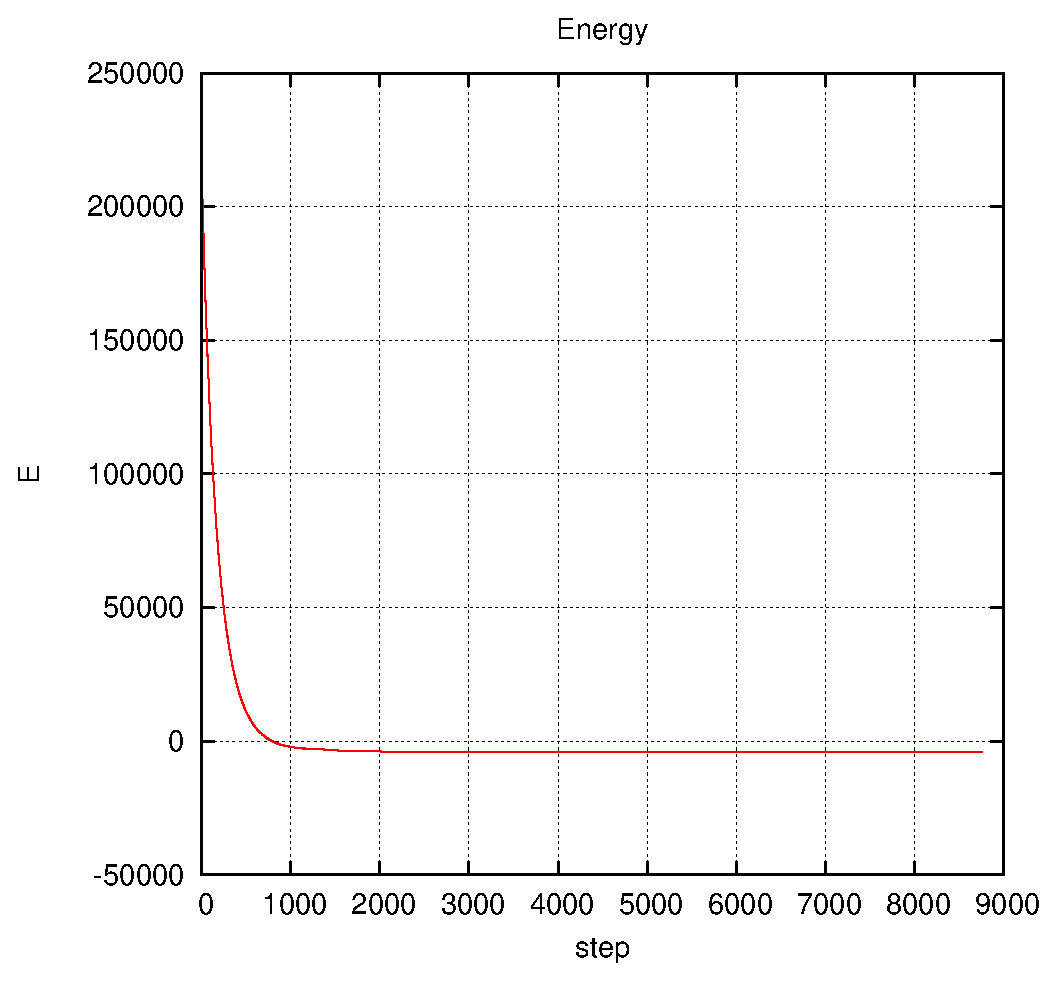
\includegraphics[scale=0.7]{E_SD_500.eps}
				\caption{andameto dell'energia durante lo Steepest Descent per il campione composto da 500 particelle. Si osserva comportamento simile alla figura \ref{fig:SD_256}}
				\label{fig:SD_500}
			\end{figure}
		Feedback utile per capire se il campione ha raggiunto valori energetici ragionevoli è osservare l'energia prima dell'aggiunta della molecola extra, dopo l'aggiunta della molecola, e al termine dello Steepest Descent:
		\begin{table}[H]
			\centering
			\begin{tabular}{l|ccc}
			\hline
		
			\hline
			\textbf{camione} & \textbf{Senza molecola} & \textbf{Con molecola} & \textbf{Risultato SD} \\
			\hline
				32	 & -218.84 	 & 999.26 	& 	-207.70 \\
				108 & 	-861.04	 & 	8524.84 & 	-852.14 \\
				256 & 	-2104.42 & 	428858.58 	& -2096.39 \\
				500 & 	-4152.05 & 	214023.88	& -4144.24 \\
			\hline
		
			\hline
			\end{tabular}
		\end{table}
		è facile notare , nel nostro caso, gli scarti siano qualitativamente molto piccoli.
		% paragraph evoluzione_dell_energia_durante_lo_steepest_descent (end)
		Se hai tempo: osservazioni sui modelli molecolari
	% subsection dati_ottenuti (end)
	% section software_per_la_creazione_del_sample (end)
	\newpage
	\section{Software per il calcolo del coefficiente di diffusione e per il riscaldamento del campione} % (fold)
	\label{sec:software_per_il_calcolo_del_coefficiente_di_diffusione_e_per_il_riscaldamento_del_campione}
		Il software ``evolution\_algorithm'' è stato sviluppato per effettuare il
		calcolo del coefficiente di diffusione dell'atomo nel sito interstiziale
		del cristallo-campione prodotto con il codice precedente.\\
		Questo programma si articola in tre grossi algoritmi:
		\begin{itemize}
			\item L'implementazione della dinamica molecolare
			\item L'inserimento del Termostato Anderson per variare la temperatura
			\item Il calcolo del coefficiente di diffusione
			\item Il calcolo della pair correlation function
		\end{itemize}
		\subsection{Dinamica molecolare} % (fold)
		\label{sub:dinamica_molecolare}
			Per il calcolo della dinamica molecolare è stato 
			applicato un algoritmo di verlet nella sua forma:
			\begin{equation}
				r(t+\Delta t)= r(t) +v(t) \Delta t +\frac{f(t)}{2 m} \Delta t^2
			\end{equation}
			\begin{equation}
				v(t+\Delta t) = v(t) + \frac{f(t+\Delta t)+ f(t)}{2 m} \Delta t
			\end{equation}
		% subsection dinamica_molecolare (end)
		\subsection{Coefficiente di diffusione} % (fold)
		\label{sub:coefficiente_di_diffusione}
			Visto il tipo di algoritmo implementato e la conseguente più facile 
			reperibilità dell'informazione sulle velocità delle particelle 
			piuttosto che il loro scostamento quadratico medio abbiamo preferito
			implementare il calcolo di questo valore attraverso la relazione di 
			Green-Kubo invece di quella classica di Einstein. Queste due relazioni
			sono del tutto equivalenti solo che la Green-Kubo ci permette di 
			accedere al coefficiente di diffusione attraverso il calcolo della 
			funzione di autocorrelazione delle velocità, operazione che ci risulta 
			molto più semplice.\\
			Partendo da:
			\begin{align*}
				2 D & = \lim_{t\rightarrow \infty} \frac{\partial\left < x^2(t)\right>}{\partial t}\\
				x(t) &= \left(\int_{0}^{t} v_x(t')dt'\right)^2 \\
				&= 2 \int_{0}^{t} \int_{0}^{t'} <v_x(t')v_x(t''>dt'dt''
			\end{align*}
			possiamo dedurre che:
			\begin{equation}
				D = \int_{0}^{\infty} d\tau <v_x(\tau)v_x(0)>
			\end{equation}
			relazione da noi implementata dopo essere stata scalata in 3 dimensioni.
		% subsection coefficiente_di_diffusione (end)
		\subsection*{Pair correaltion function} % (fold)
		\label{sub:pair_correaltion_function}
			Il calcolo della $g(r)$ è stato implementato per permettere un analisi
			qualitativa dello stato del campione.
		% subsection pair_correaltion_function (end)
		\subsection{Dati Ottenuti} % (fold)
		\label{sub:dati_ottenuti_2}
			le misure sono state effettuate portando prima il campione alla temperatura desiderata e poi facendovi la misura di diffusione a temperatura costante. In
			Figura \ref{mis1} vediamo, a titolo esemplificativo i dati riguardanti la prima misura a temperatura 0.\\
			I primi set di valori raccolti erano errati di ordini di grandezza a causa del moto del centro di massa del campione che veniva introdotto durante innalzamento della temperatura. Tale errore è stato risolto introducendo nell'algoritmo la rimozione, dopo il caricamento delle velocità, della velocità del centro di massa.
			Essendo la velocità del centro di massa, dopo un riscaldamento, di ordini vicini a $\sim 10^{-2}$ questo causa una diminuzione di energia cinetica (e conseguentemente di temperatura) dell'ordine $\sim 10^{-4}$ che abbiamo considerato trascurabile.\\
			I valori di diffusione raccolti alla fine sono stati:
			\begin{table}[H]
				\centering
			
				\begin{tabular}{l|c}
				\hline
			
				\hline
				\textbf{Temperatura} & \textbf{D} \\
				\hline
					$0.00$ &	$1.75*10^{-8}$\\
					$0.02$ &	$5.21*10^{-5}$\\
					$0.05$ &	$3.76*10^{-3}$\\
					$0.08$ &	$9.41*10^{-4}$\\
					$0.15$ &	$1.31*10^{-2}$\\
					$0.20$ &	$1.45*10^{-2}$\\
					$0.30$ &	$1.25*10^{-2}$\\
					$0.35$ &	$1.51*10^{-2}$\\
					$0.45$ &	$3.34*10^{-2}$\\
				\hline
			
				\hline
				\end{tabular}
			\end{table}
			per una finestra da 10000 campioni (eccetto l'ultimo dove sono stati utilizzati solo mille campioni) di autocorrelazione su 100000 step temporali in un ensamble microcanonico.
			\begin{figure}[H]
				\centering
				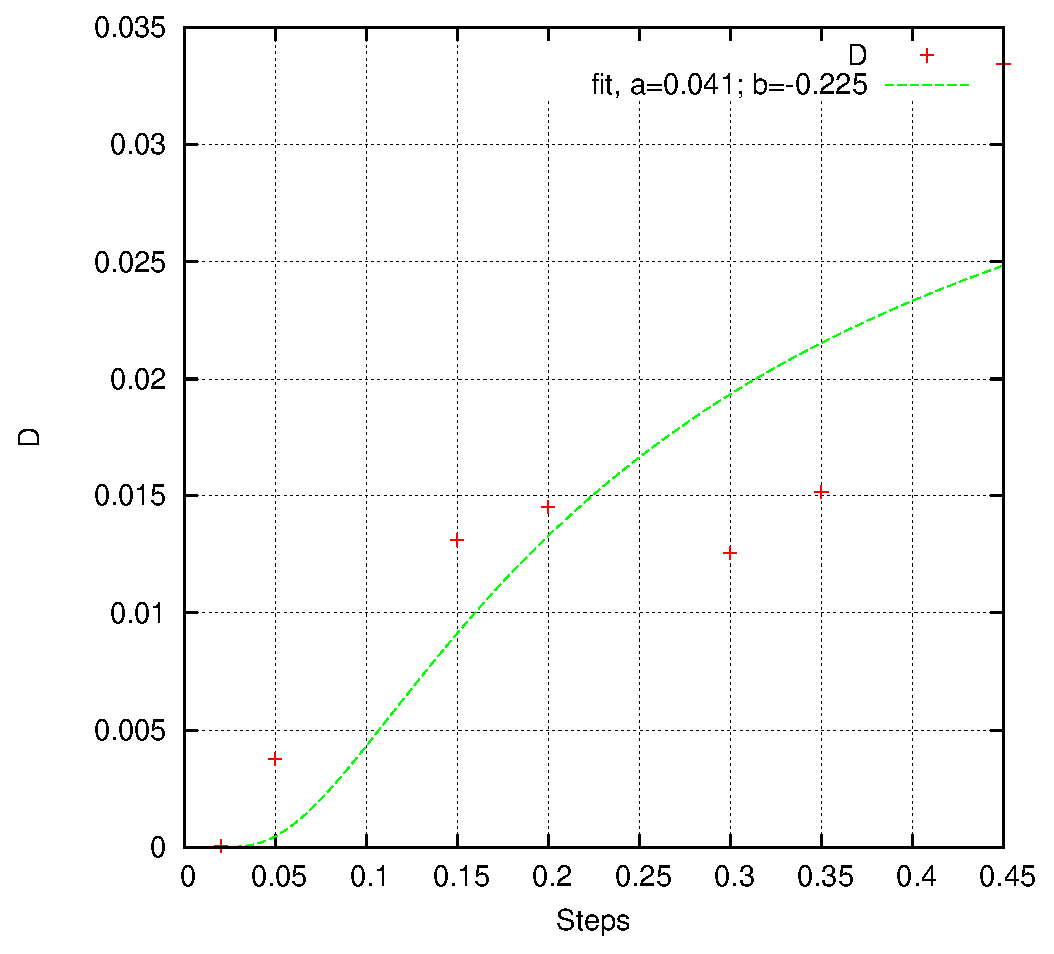
\includegraphics[scale=0.7]{fit.eps}
				\caption{Tabella precedente con Fit sui dati rilevati. a=$D_0$,b=$Q$}
				\label{fig:figure1}
			\end{figure}
			
			I Punti raccolti non sono molto compatibili con il fit pertanto si è cercato, senza però ottenere risultati soddisfacenti di migliorare la raccolta dei punti, provando ad allargare e rimpicciolire la finestra di autocorrelazione, aumentando i punti di analisi, provando a fare lo studio su ensamble differenti. Si sono visti benefici al ridursi della finestra di autocorrelazione con conseguente aumento di punti su cui veniva fatta la media di ciascuna autocorrelazione, sfortunatamente siamo giunti a questa conclusione troppo tardi; .\\
			Visto il parziale insuccesso la nostra analisi si è fermata qui.

			\begin{figure}[H]
				\centering
				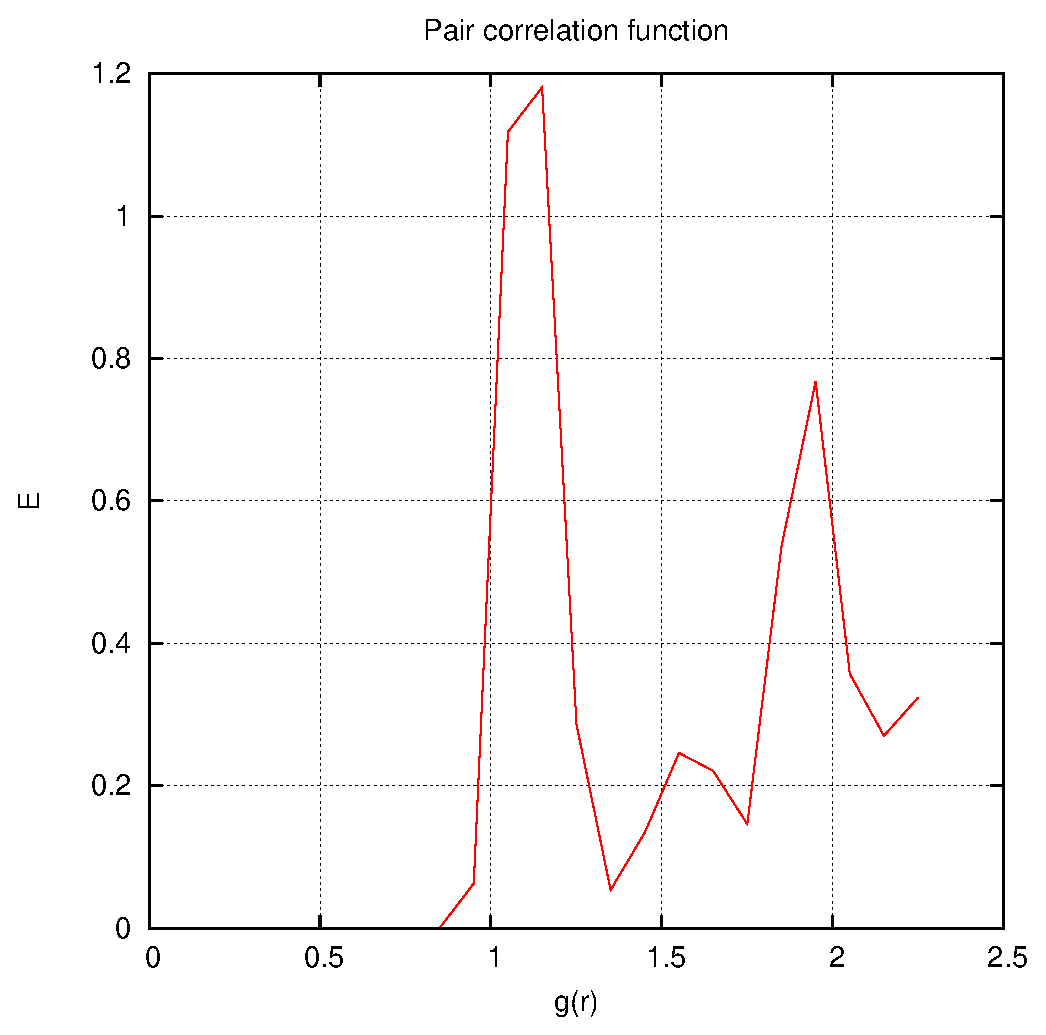
\includegraphics[scale=0.7]{gr_0_45.eps}
				\caption{funzione di autocorrelazione a $T^*=0.45$, permane lo stato solido ma stiamo andando verso uno stato liquido, è coerente con l'aumento del coefficiente di diffusione}
				\label{fig:gr045}
			\end{figure}

			\begin{figure}[H]
				\centering
				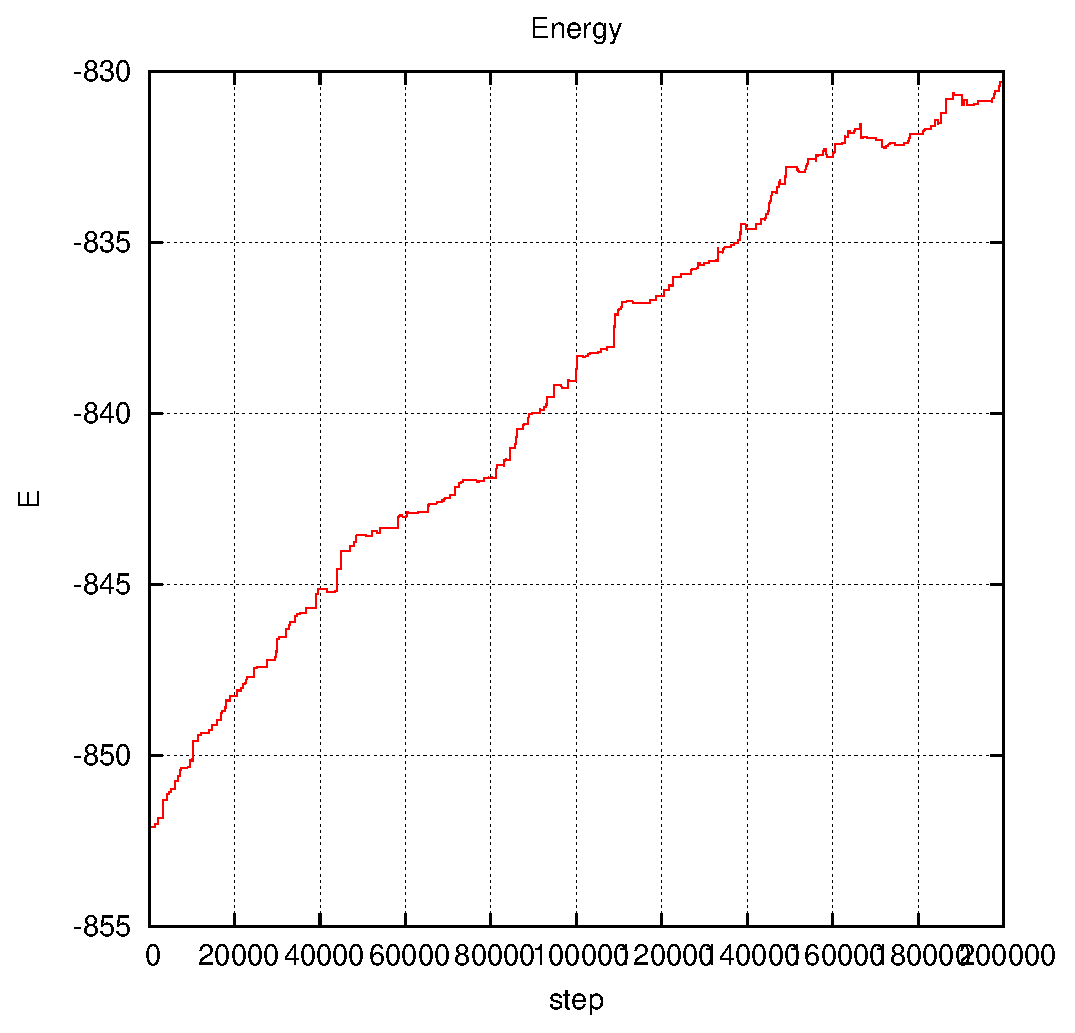
\includegraphics[scale=0.7]{Energy_evolution.eps}
				\caption{Evoluzione dell'energia totale durante un aumento di temperatura, si riconoscono i tipici scalini dovuti alle interazioni delle molecole con il termostato}
			\end{figure}


				\begin{sidewaysfigure}
					\label{mis1}
					\centering%
					\subfigure[Energia durante la simulazione, oscillazioni sulla decima cifra decimale]%
					{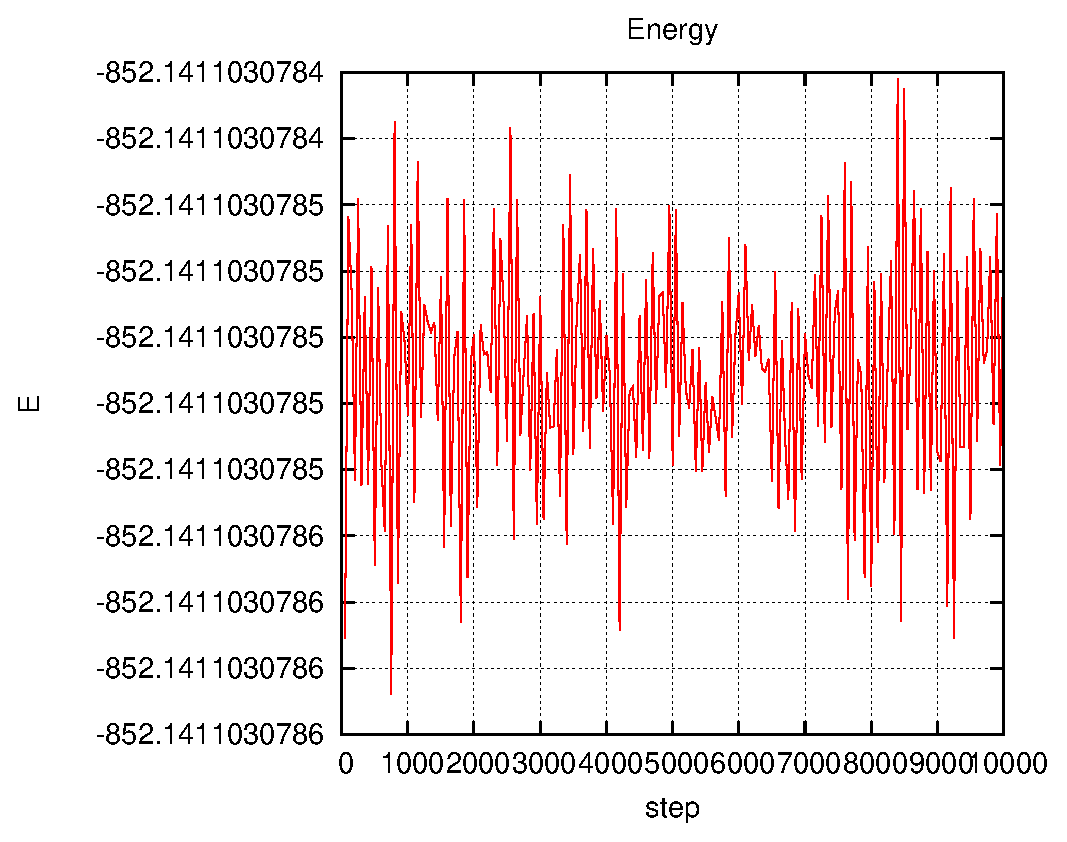
\includegraphics[scale=0.5]{Energy_evolution_0.eps}}
					\qquad\qquad
					\subfigure[picchi a 1.12, 1.58...]%
					{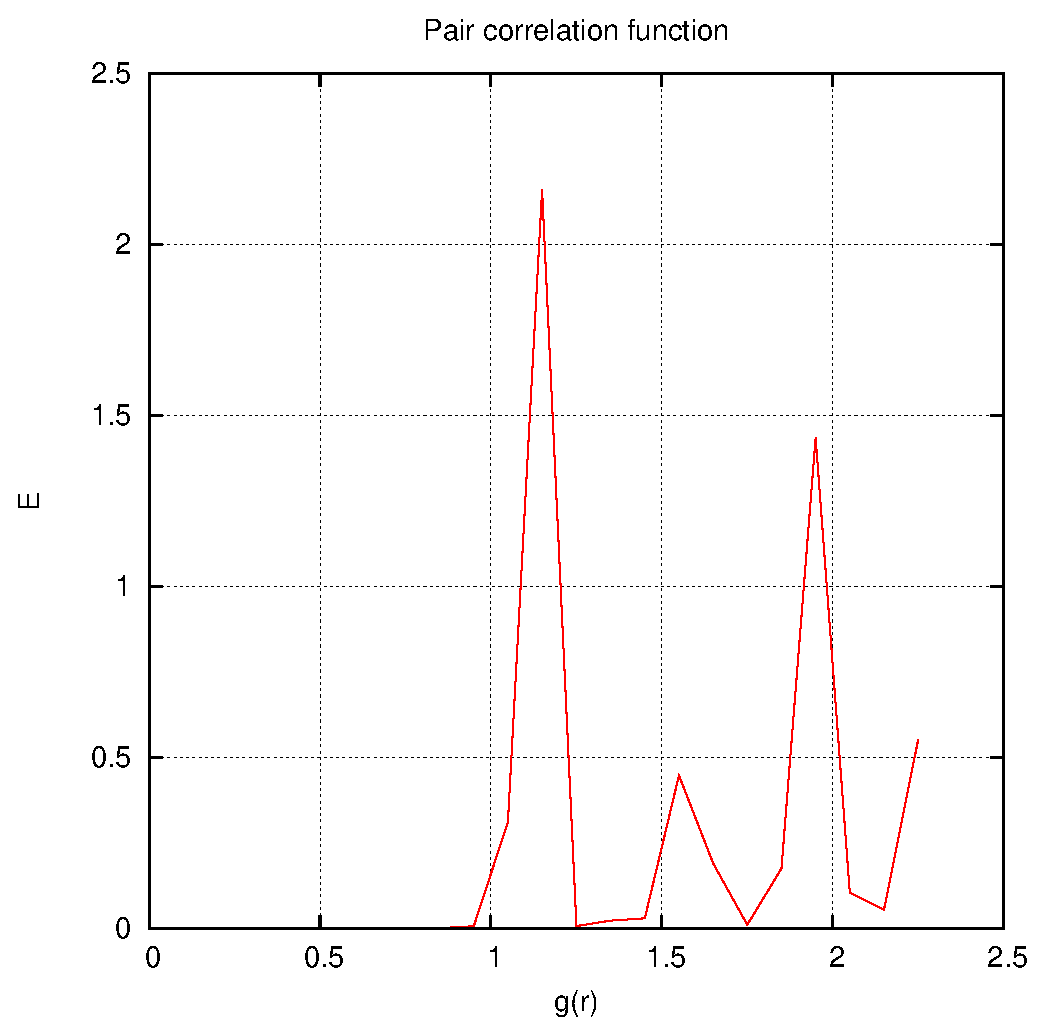
\includegraphics[scale=0.5]{gr_0.eps}}\qquad\qquad
					\subfigure[temperatura costante durante la presa dati]%
					{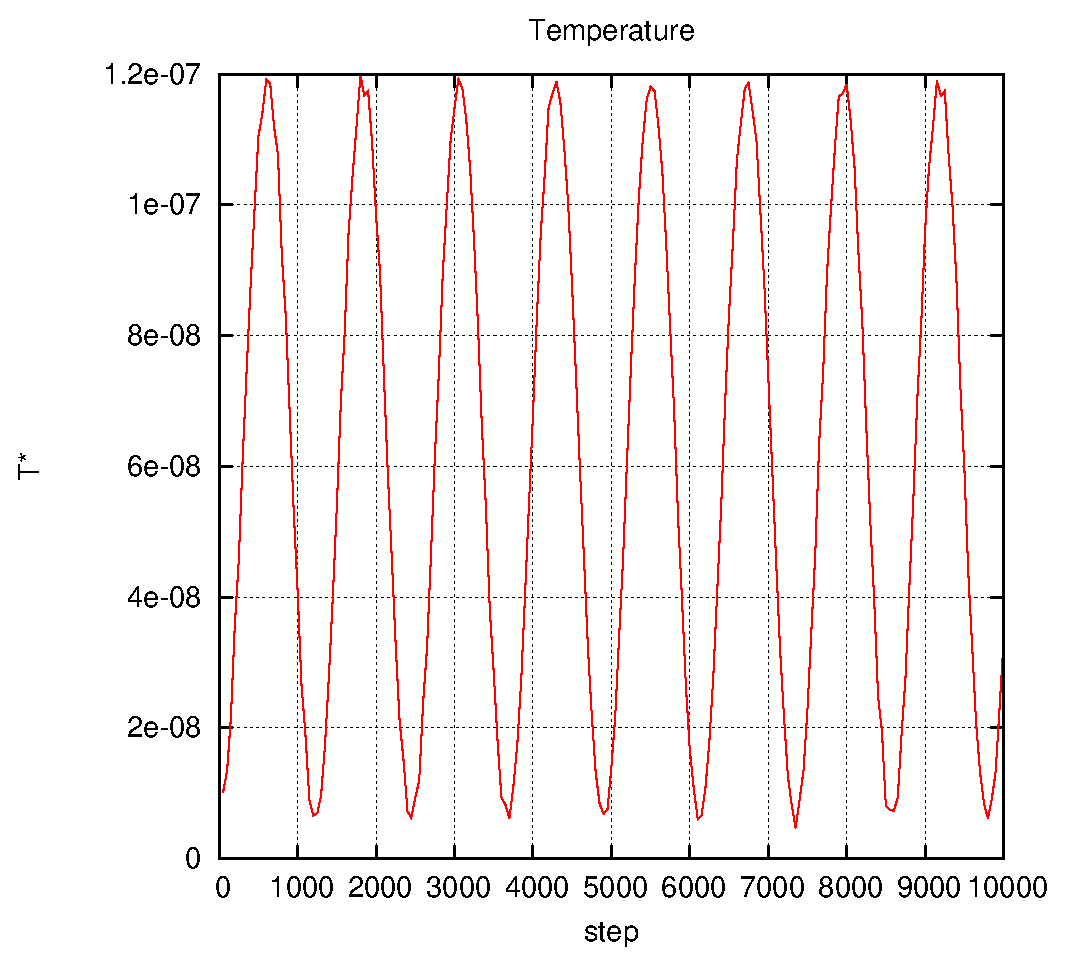
\includegraphics[scale=0.5]{Temperature_evolution_0.eps}}
					\caption{Questi sono i dati relativi alla prima misura presa a T=0 per il campione composto da 108+1 particelle. Si nota in particolare la g(r) molto piccata che sta ad indicare un quasi perfetto stato solido e la temperatura che ha un evoluzione armonica dovuta probabilmente al potenziale scelto e ai piccoli scostamenti permessi alle molecole}
				\end{sidewaysfigure}
			% paragraph prima_misura_t_0 (end)
		% subsection dati_ottenuti (end)
	% section software_per_il_calcolo_del_coefficiente_di_diffusione_e_per_il_riscaldamento_del_campione (end)
	\newpage
	\section{Conclusioni} % (fold)
	\label{sec:conclusioni}
	Il primo algoritmo ha prodotto i risultati desiderati creando campioni coerenti con quanto desiderato ed e minimizzando in maniera opportuna l'energia attraverso uno Steepest Descent; è possibile fare affermazioni qualitative sul risultato osservando come l'energia raggiunta dopo il rilassamento sia paragonabile a quella di campione senza sito interstiziale.\\
	Il secondo algoritmo, nonostante l'apparente correttezza teorica, non è stato capace di produrre i risultati desiderati. Qualitativamente i valori ottenuti seguono un andamento corretto ma quantitativamente i fit si discostano troppo dai valori misurati. I tentativi di miglioramento hanno dato risultati diminuendo la dimensione della finestra di autocorrelazione ovvero mediando D su più misure.
	% section conclusioni (end)
\end{document}